%%%%%%%%%%%%%%%%%%%%%%%%%%%%%%%%%%%%%%%%%%%%%%%%%%%%%%%%%%%%%%%%%%%%%%%%%%%%%%%%%%%%%%%%%%%%%%%%%%%%
% ==================================================================================================
% --------------------------------------------------------------------------------------------------
\chapter{Methodology}
In this section we motivate and introduce the proposed model, and explore its parametrization. Wherever possible, concepts related to segmentation and classification will be described in their most general sense, since many of the these may also apply to other image analysis and machine learning tasks.
%%%%%%%%%%%%%%%%%%%%%%%%%%%%%%%%%%%%%%%%%%%%%%%%%%%%%%%%%%%%%%%%%%%%%%%%%%%%%%%%%%%%%%%%%%%%%%%%%%%%
\section{Model Design}\label{s:modelconcept}
As suggested in \S\ \ref{ss:priorproposed}, three general paradigms have emerged for segmentation of brain MRI. The first and most popular is the pipeline, in which sub-tasks are completed in sequence, such as: pre-processing, classification, post-processing. This approach permits a flexible model definition which can incorporate existing algorithms for individual steps. Most thresholding and classic supervised models fall under this category. The main drawback of this approach is that some steps could be improved by the results of downstream steps. For example, tissue classifying modules typically assume that the bias field is already corrected, but bias field estimation can be more accurate if the tissue segmentation is known.
\par
The second paradigm, a unified generative model, aims to solve this chicken-egg problem. The segmentation is parameterized in one integrated probabilistic model, which often combines the input images with tissue prior probability images, a bias field model, and smoothness terms. Parameters of each sub-model are estimated using several expectation maximization iterations before the final segmentation is inferred. The challenges to this approach include balancing model complexity with estimability, robust convergence issues, and reduced ability to include external tools.
\par
The final paradigm, deep learning, uses error back-propagation to update thousands of parameters in a large, relatively unstructured model mapping the input MRI to the output segmentation image. Using so-called ``end-to-end'' training, there is no guarantee that the usual sub-components (e.g. bias field, tissue graylevel distributions, etc.) will be estimated, though such elements could be expected to develop in the internal relationships if they are relevant to the task at hand. Most deep learning models still require standardization in space and graylevel, and more importantly, large training datasets -- which are rare in medical imaging.
\par
For several reasons, the supervised pipeline approach was selected for this work.
First, preliminary work drawing on existing algorithms \cite{Khademi2014,Schmidt2015} showed the feasibility of several relatively simple thresholding methods, which confer robustness through simplicity.
Second, the parametric assumptions required by unified probabilistic models may be challenged by data from multiple sources \cite{VanLeemput2001}.
Third, only a small number of training cases were available during initial development, which limited the feasibility of deep learning approaches.
Finally, time constraints favoured the incorporation of existing tools to address challenges like bias correction and image registration, which would have been otherwise difficult to develop in a unified model.
% ==================================================================================================
\subsection{Features}
Many FLAIR-only WMH segmentation algorithms use a thresholding technique: map a single graylevel feature directly to a class or class probability (e.g. ``healthy'' or ``lesion''). Such models often have complex methods of deriving this mapping (e.g. using mixture model parameters \cite{Roura2015}, histogram features \cite{Yoo2014}, or conditional edge probability \cite{Knight2016}), but the final rule is applied equally to the entire graylevel image, usually the FLAIR sequence. The most common challenge for these methods is a high number of false positives (c.f. \S\ \ref{ss:metrics} for definitions), since several artifacts and GM can overlap the WMH intensity distribution. As a result, nearly all previously proposed thresholding algorithms employ heuristic ``false positive reduction'' (FPR) rules as post-processing to remove these errors.
\par
% Need to introduce registration \& MNI space earlier (\cite{Evans1993})
Preliminary investigations sought to characterize the spatial distribution of false positives, in order to explore possible FPR rules. Using a database of 96 FLAIR images in MNI space (c.f. \S\ \ref{ss:data} for details), the optimal threshold for each image was calculated%
\footnote{The \texttt{fminsearch} function in Matlab maximized the similarity index with respect to the manual segmentation.}
and used to generate binary class images ($0 =$ healthy, $1 =$ lesion). Comparing these results with the manual segmentations, the average distribution of true positives (TP), false positives (FP), and false negatives (FN) was computed, as shown in Figure \ref{fig:thropt-tpfpfn}. The median optimal similarity index (SI) was 0.36.
\begin{figure}[h]
  \centering
  \begin{subfigureside}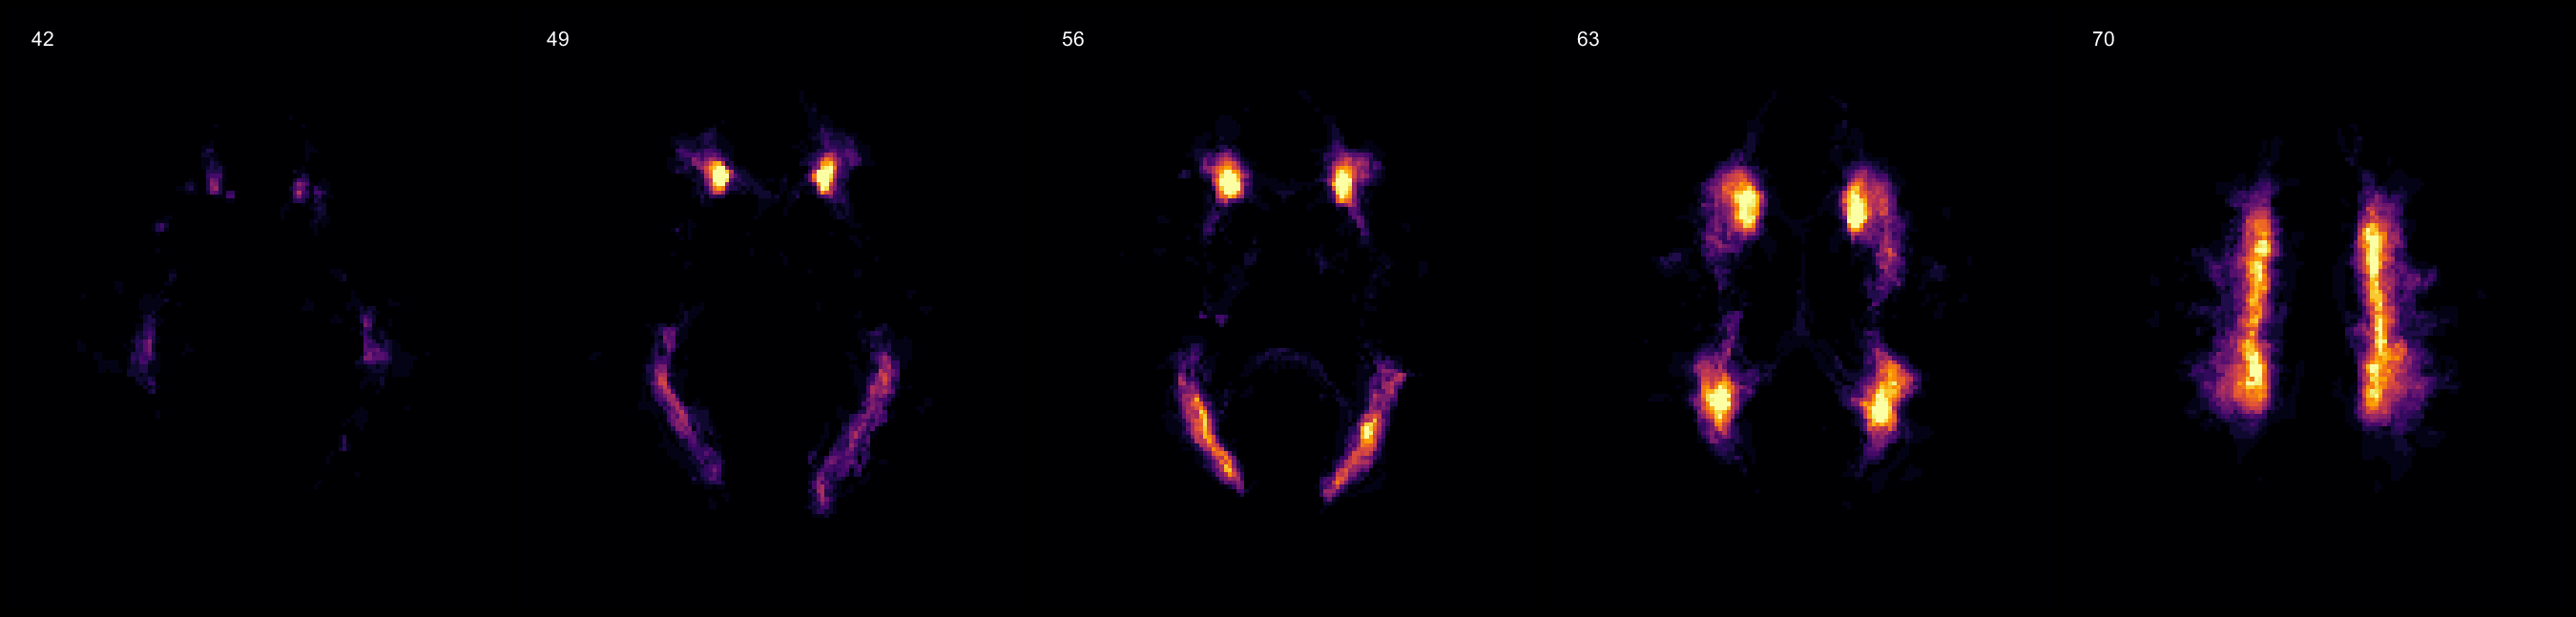
\includegraphics[height=\sliceheight]{rawthropt-tp.png} 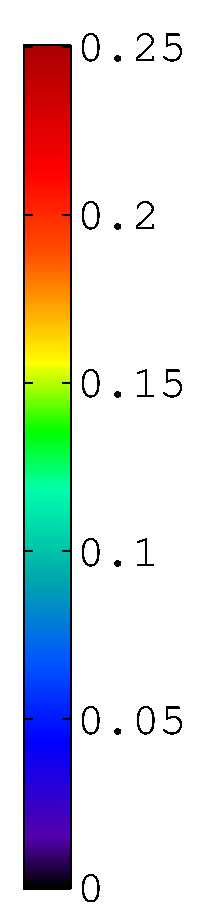
\includegraphics[height=\sliceheight]{cbar-NIH3-0-025}\end{subfigureside}\\[0.5em]
  \begin{subfigureside}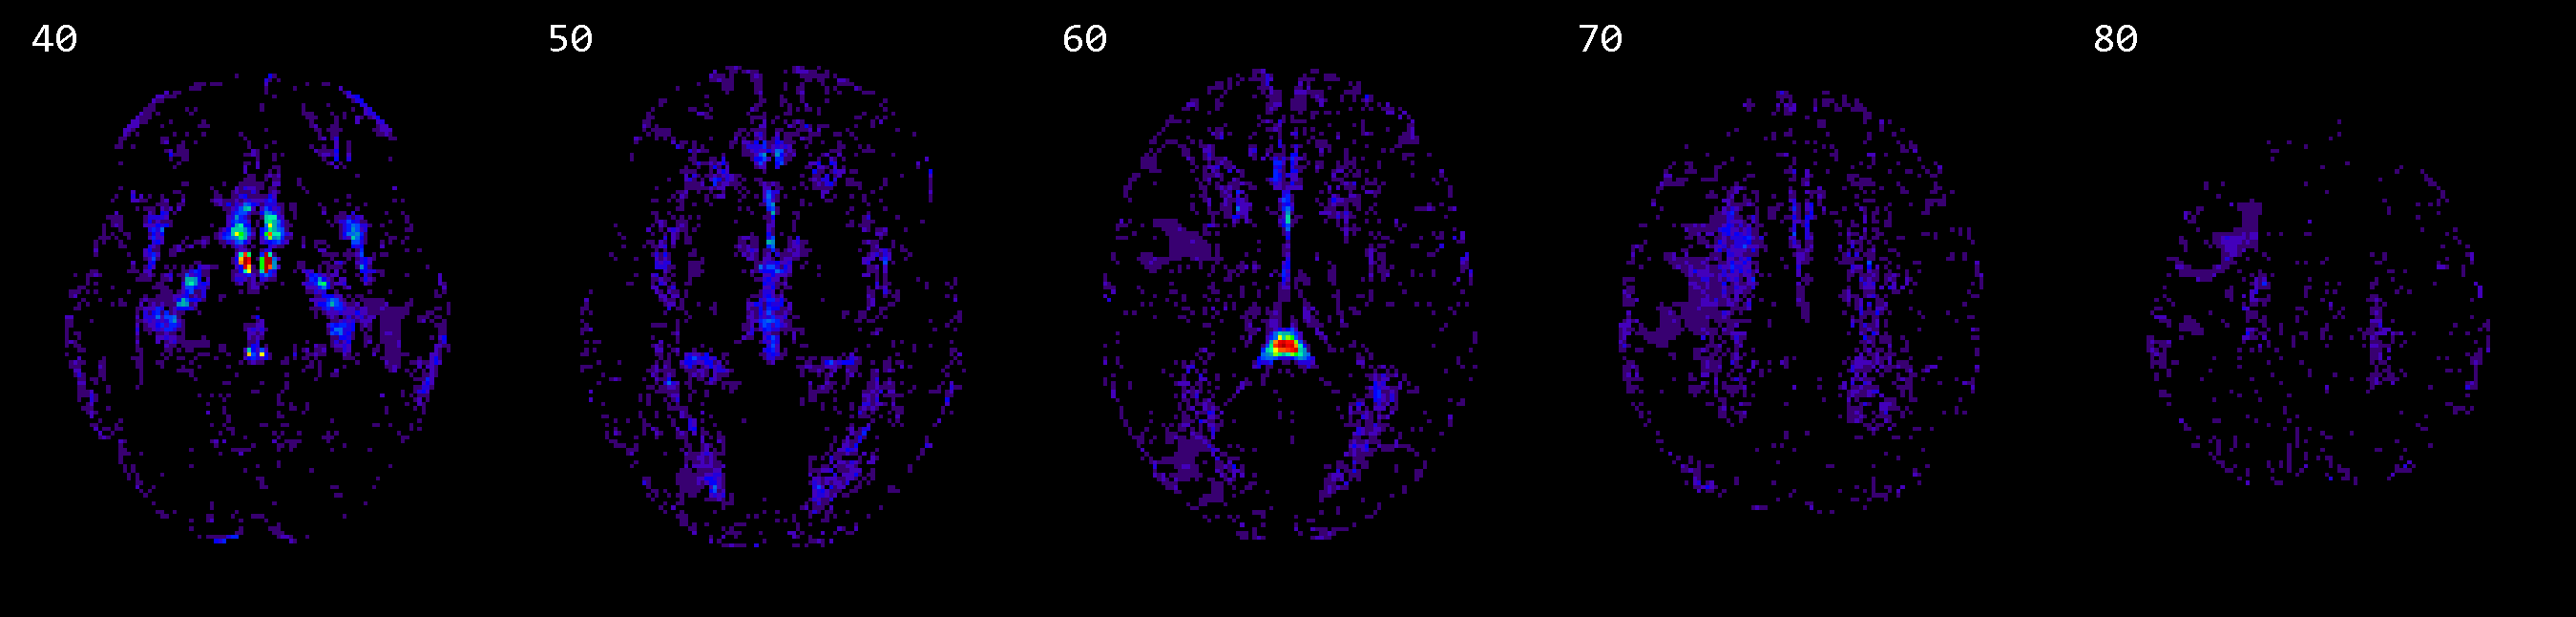
\includegraphics[height=\sliceheight]{rawthropt-fp.png} 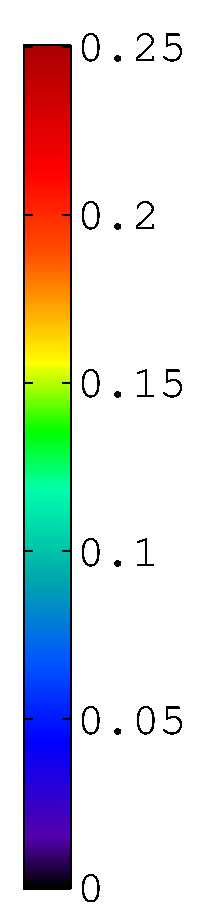
\includegraphics[height=\sliceheight]{cbar-NIH3-0-025}\end{subfigureside}\\[0.5em]
  \begin{subfigureside}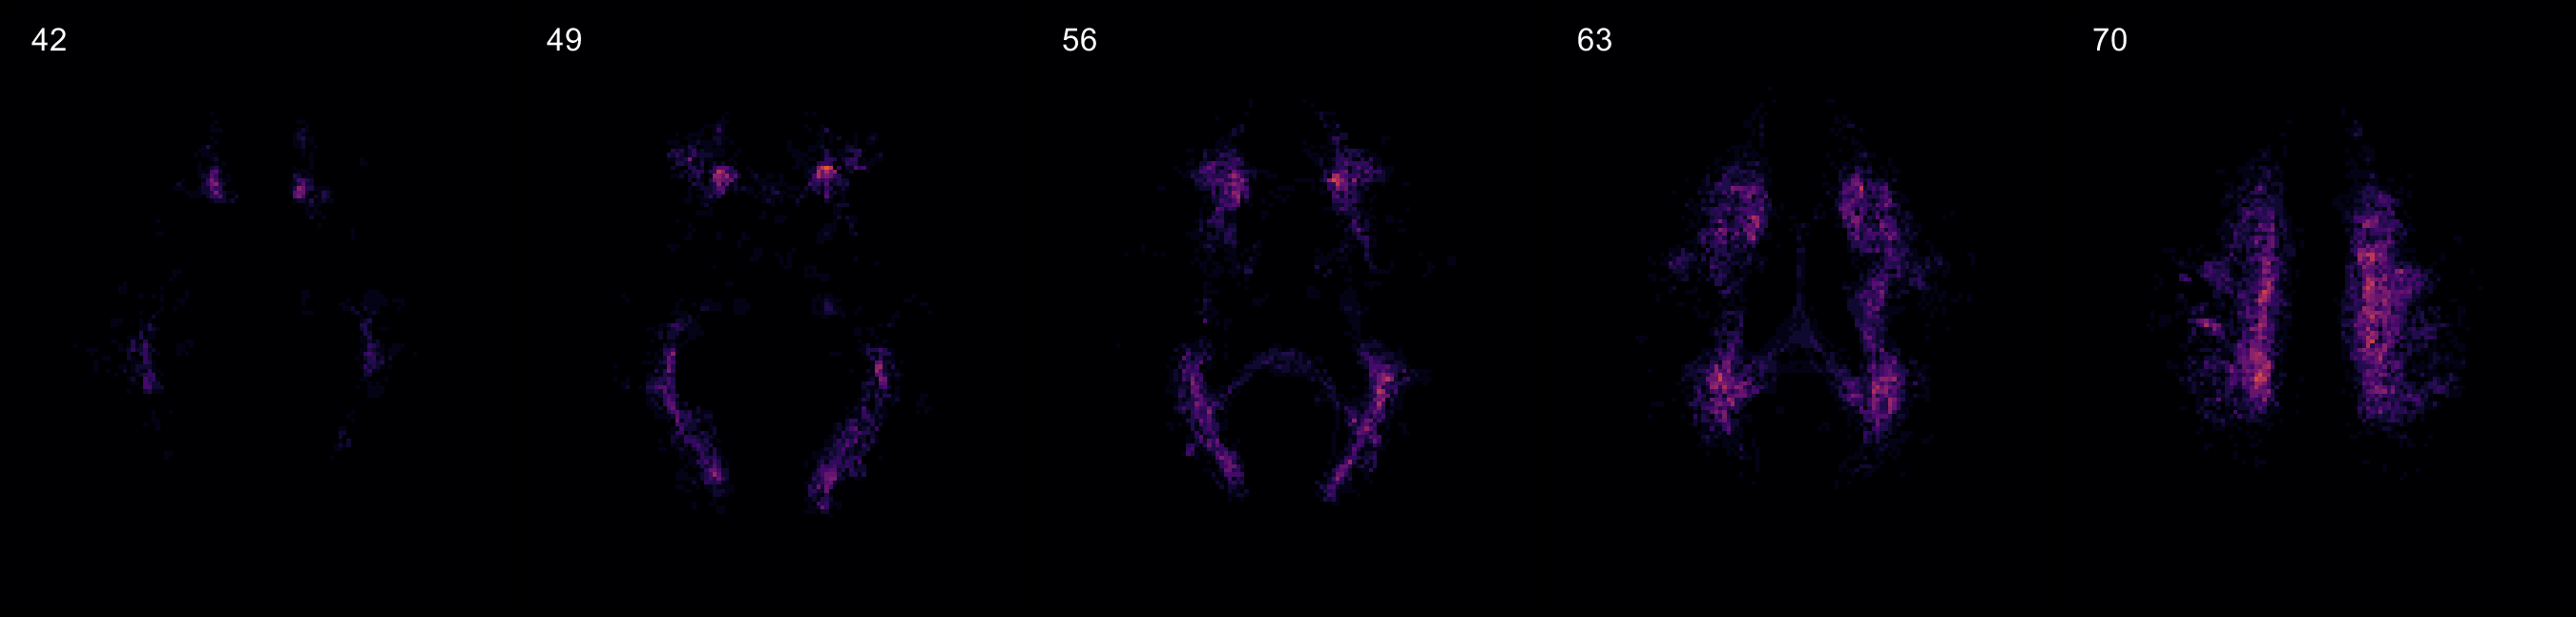
\includegraphics[height=\sliceheight]{rawthropt-fn.png} 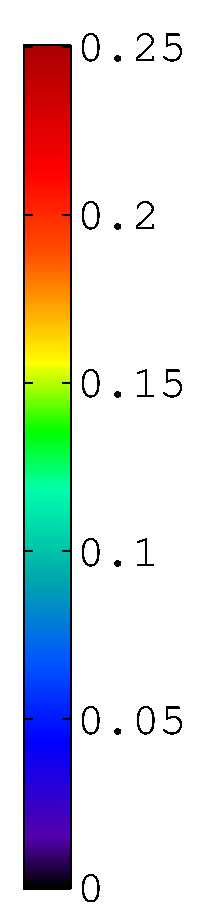
\includegraphics[height=\sliceheight]{cbar-NIH3-0-025}\end{subfigureside}\\[0.5em]
  \caption{Distributions of (a) TP, (b) FP, and (c) FN in 96 FLAIR MRI, following supervised optimal thresholding in MNI space.}
  \label{fig:thropt-tpfpfn}
\end{figure}
\par
Evidently, even if an optimal threshold could be estimated for these data, a high proportion of FP and FN would be incurred. Yet in Figure \ref{fig:thropt-tpfpfn} there are regular and distinct spatial distributions of these errors. Moreover, is it has been suggested that there is regional heterogeneity in relaxation rates of brain tissues \cite{Sled2004}, and that WML intensity depends in part on location \cite{Stevenson2000,Harmouche2015}. This implies that spatial coordinates would be useful features for WMH segmentation, especially when incorporated into the main classification model (i.e. not as post-processing). Indeed such features have previously been used \cite{Anbeek2004,Anbeek2005,Dyrby2008,Griffanti2016,Dadar2017}.
\par
Spatial features could be used with FLAIR intensities in supervised classification models like K-NN, SVM, RF, etc. However, such models treat all features equally, which can lead to artifacts in the decision boundary that contradict prior knowledge. For example, in spatial locations which do not observe any lesions during training, the optimized model may learn to never predict the lesion class, regardless of graylevel features. Similarly, there is no guarantee that FLAIR graylevels will map monotonically to the lesion class, as would be expected. Therefore, spatial features should be treated differently.
% ==================================================================================================
\subsection{Overview}
The proposed pipeline can be summarized as follows. Pre-processing steps will aim to correct any bias field effect and standardize spatial coordinates. The classification model will employ FLAIR intensities and spatial features to give the initial segmentation. Since most classification models assume features are drawn from a consistent distribution, a graylevel standardization step is appended to the pre-processing. Post-processing steps will generally aim to improve segmentation performance. This pipeline is illustrated in Figure \ref{fig:pipeline}. Next, the proposed classification model is developed.
\begin{figure}
  \centering\scalebox{0.65}{\pgfdeclarelayer{background}
\pgfdeclarelayer{foreground}
\pgfsetlayers{background,main,foreground}
\tikzset{%
  arrow/.style = { ->, >=Latex,  very thick, rounded corners, draw = #1!60!white },
  tbox/.style  = { fill = white, draw = #1!60!white, very thick, align = center }
}
\newcommand*{\textbox}[6]{%
  \node[tbox=#5,minimum width=#3cm,minimum height=#4cm]at(#1,#2){#6};
}

\newcommand*{\ix}{0.8}\newcommand*{\ixx}{1.6}
\newcommand*{\iy}{1}  \newcommand*{\iyy}{2}
\newcommand*{\pw}{1.5}
\newcommand*{\fw}{0.3}

% --------------------------------------------------------------------------------------------------
\begin{tikzpicture}
    \useasboundingbox(0.0, 0.0) rectangle (24.0,  2.0);
    \draw[black!30!white,rounded corners,very thick](00.0, 00.0) rectangle (24.0,  2.0);
    \textbox{ 2.0}{ 1.0}{3}{1}{black} {FLAIR MRI}
    \textbox{ 6.0}{ 1.0}{3}{1}{blue}  {Bias Correction\\\& Registration}
    \textbox{10.0}{ 1.0}{3}{1}{violet}{Graylevel\\Standardization}
    \textbox{14.0}{ 1.0}{3}{1}{red}   {Lesion\\Classification}
    \textbox{18.0}{ 1.0}{3}{1}{orange}{Post-Processing}
    \textbox{22.0}{ 1.0}{3}{1}{black} {Label Image}
    \draw[arrow={black}  ]( 3.5, 1.0)--( 4.5, 1.0);
    \draw[arrow={black}  ]( 7.5, 1.0)--( 8.5, 1.0);
    \draw[arrow={black}  ](11.5, 1.0)--(12.5, 1.0);
    \draw[arrow={black}  ](15.5, 1.0)--(16.5, 1.0);
    \draw[arrow={black}  ](19.5, 1.0)--(20.5, 1.0);
%    \draw[arrow={black} ]( 3.5, 1.0)--( 4.5, 1.0);
%    \draw[arrow={blue}  ]( 7.5, 1.0)--( 8.5, 1.0);
%    \draw[arrow={violet}](11.5, 1.0)--(12.5, 1.0);
%    \draw[arrow={red}   ](15.5, 1.0)--(16.5, 1.0);
%    \draw[arrow={orange}](19.5, 1.0)--(20.5, 1.0);
\end{tikzpicture}}
  \caption{Overview of the necessary processing steps.}
  \label{fig:pipeline}
\end{figure}
% address challenges here?
%- overlapping distributions \& hyperintense artifacts: spatial parametrization
%- bias field: correct beforehand
%- DAWM \& PVA: maintain probabilistic output 
%- image variability: graylevel standardization, image registration, spatial parametrization
%However, it has been suggested that there is regional heterogeneity in relaxation rates of brain tissues \cite{Sled2004}, and that WMH intensity depends in part on location \cite{Stevenson2000}.
%Many of the previously proposed WMH segmentation algorithms predict the class of a voxel without any spatial information. In the absence of spatial information, 
%The work by \citeauthor{Khademi2012} \cite{Khademi2012,Khademi2014,Khademi2015} was particularly promising, since it overcame many of the usual requirements. These include: the use of multiple MRI modalities, which are not always available; image registration to a common space, which is never perfect and introduces interpolation artifact; the use of training data, which is difficult to find; and assumed Gaussian distribution of tissue graylevels, which is rarely valid.
%Assumptions which many models make, and whether they are wrong:
%%- parametric modelling of graylevel distributions: with single Gaussians: almost certainly wrong. Confounding factors: PVA, parallel MRI signals, motion artifacts, 
%%The most recent implementation of the EM-fit mixture model by \citeauthor{Ashburner2005} in \cite{Ashburner2005} permits a user-specified number of Gaussian distributions for each tissue class, 
%However, 
%\begin{figure}
%  \centering
%  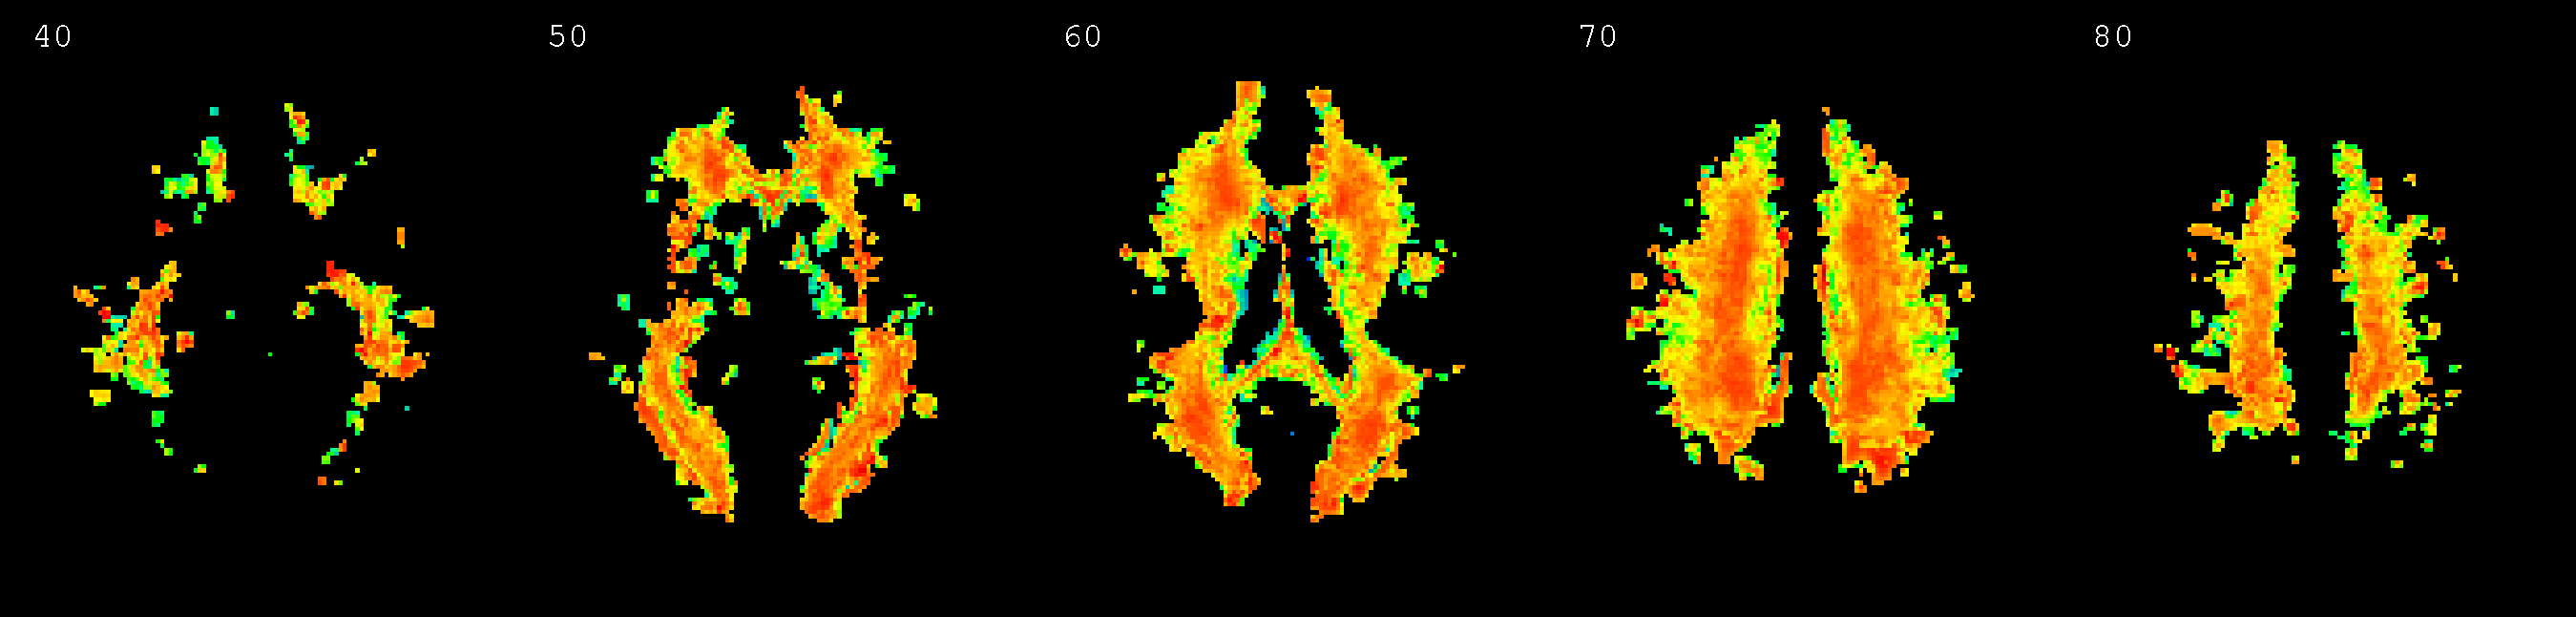
\includegraphics[height=\sliceheight]{meangray-c1.png}
%  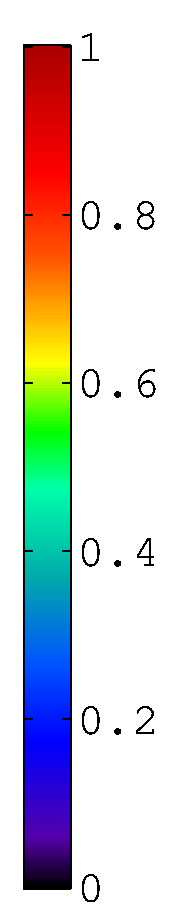
\includegraphics[height=\sliceheight]{cbar-NIH3-0-1.eps}
%  \caption{Mean lesion class graylevel after standardization in 96 coregistered FLAIR MRI.}
%  \label{fig:meangray-c1}
%\end{figure}
%%%%%%%%%%%%%%%%%%%%%%%%%%%%%%%%%%%%%%%%%%%%%%%%%%%%%%%%%%%%%%%%%%%%%%%%%%%%%%%%%%%%%%%%%%%%%%%%%%%%
\section{Voxel-Wise Logistic Regression}\label{s:vlr}
This section presents the proposed classification model: Voxel-wise Logistic Regression (VLR). The VLR model solves the problem of differential treatment for spatial and graylevel features, and produces uniquely interpretable parameters following training. The model is inspired by the LPA algorithm in the LST toolbox for SPM by \citeauthor{Schmidt2015} \cite{Schmidt2015,Schmidt2017a}%
\footnote{This algorithm was originally understood through the Matlab code, after downloading the toolbox. Section 6.1 of \cite{Schmidt2017a}, published in \citeyear{Schmidt2017a}, provides more details.}%
, however, novel methods of model parametrization and estimation are presented here, in addition to differences in pre- and post-processing from the LPA algorithm.
\par
Logistic regression models have recently gained popularity for WMH segmentation \cite{Sweeney2013a,Sweeney2013,Schmidt2017a,Zhan2017}, and have several advantages.
First, model parameters are generally more interpretable than those in other models, permitting better design of regularizations.
Second, the simplicity of the model reduces its capacity for over-fitting. 
Third, model foundations in statistical theory allow probabilistic interpretations of the outputs, which may be helpful for quantifying marginally pathological tissues like DAWM.
The major drawback of logistic models for WMH segmentation is that standardization of graylevels is required.
\par
In the two class formulation, the lesion class is denoted $c=1$, and the healthy class $c=0$. The probability of the lesion class, given a set of features $\by = [1,y^1,\dots,y^\K]^T$ is modelled by a logistic function, parameterized by a vector of feature weights $\bb = [\b^0,\b^1,\dots,\b^\K]^T$,
\begin{equation}
  P(c=1\mid\by,\bb) = \frac{1}{1+e^{-\eta}},\qquad\eta = \bb^T\by.
  \label{eq:lrmodel}
\end{equation}
This probability -- the estimated lesion class label -- is denoted $\hat{c} = P(c=1\mid\by,\bb) \in [0,1]$. Considering the spatial location $x = [\xxx]$, the label image is defined as $\hat{C}(x) = P(C(x)=1\mid\bm{Y}(x),\bb)$.
\par
Previous works have not included spatial dimensions in the logistic feature set $\by$, since $\hat{c}$ is not expected to be monotonically related to any spatial dimension. The circumvention proposed by \citeauthor{Schmidt2015} is to parameterize the feature weights spatially -- that is $\bb\rightarrow\bb(x)$,
\begin{equation}
  \hat{C}(x) = \frac{1}{1+e^{-\eta(x)}},\qquad\eta = \bb(x)^T\bm{Y}(x).
  \label{eq:eq:vlrmodel}
\end{equation}
In this way, the characteristics of the logistic regression model are maintained with respect to graylevel features, but spatial features can have more complex relationships with the output. A second pre-processing step, however, is now required: standardization of spatial dimensions -- i.e. registration of the input image to a consistent target -- so that the same voxel in every input image corresponds to the same brain region. Training the VLR model then yields a unique vector $\bb$ for each voxel, or equivalently, one complete image for each parameter. Such ``parameter images'', as they will be called, are then readily interpretable and can be regularized intuitively.
%Regarding notation in the following subsections: 1) the $(x)$ is omitted here, for clarity, and 2) while only the FLAIR graylevels are used in this implementation, the $\by$ notation is maintained below for compatibility with arbitrary input feature images.
%This approach is similar to the work by \citeauthor{Harmouche2015} \cite{Harmouche2015}, wherein different mixture models are fitted for each of 6 different anatomical regions. Since no group statistics are needed in the current model, anatomical parcellations can be replaced by a smooth spatial parametrization.
%The assumptions of this model include the following:
%\begin{itemize}[itemsep=0pt]
%  \item only 2 tissues classes are modelled: WMH and healthy brain tissue;
%  \item image graylevel(s) and spatial location are sufficient features to discriminate the two classes;
%  \item in each voxel, the WMH class is monotonically separable from the healthy class by graylevel(s)
%\end{itemize}
% ==================================================================================================
\subsection{Model Fitting}\label{ss:modelfitting}
Fitting the VLR model involves estimating $\bb$ for each voxel $x$. This requires some training data: feature vectors from a population of $N$ observations $\bY = \{\by_1,\dots,\by_\N\}$, and the corresponding labels $\C = \{c_1,\dots,c_\N\}$. Typically, parameter estimation involves maximizing the likelihood of the model, given this data -- i.e. maximum likelihood estimation (MLE).
\par
Three major challenges emerge during model fitting. These challenges involve contradictions between prior knowledge and the fitted model using the available training data. That is, these challenges could all be overcome by a more complete training set, but this is usually not available. The three challenges are:
\begin{enumerate}
  \item \label{chmle:separable} \textbf{Separable classes:} 
  When data from two classes are perfectly separable, the MLE-fitted logistic model can approach a step-function -- i.e. $\b^k\rightarrow+\infty$. This implies that on either side of a specific graylevel threshold, the model is either 100\% confident in predicting the healthy class, or 100\% confident in predicting the lesion class. In fact, no threshold is ever so perfect, and instead a level of uncertainty should be maintained around the decision boundary. These two cases are illustrated in Figure \ref{fig:chmle-sep}.
  \item \label{chmle:sparse} \textbf{Sparsely observed lesion class:} 
  Since WML are often distributed in consistent locations, many brain regions contain no lesions across the entire training dataset. These voxels will be termed ``healthy training'' voxels. In some locations, this is expected (e.g. the GM, since by definition WMH manifest in the WM), while in others, our prior knowledge predicts lesions will eventually be observed (e.g. the rest of the WM). As illustrated in Figure \ref{fig:chmle-noles}, the MLE-fitted model may not maintain the ability to predict $\hat{c} = 1$ in such locations, regardless of the features. However, the ability to predict lesion should be maintained in many of these locations.
  \item \label{chmle:noisy} \textbf{Smooth parameter images:} 
  It is assumed that similar locations will contain similar training data, yielding smooth parameter images. If this assumption is sometimes invalid, parameter images could contain noise or discontinuities, creating artifacts in estimated lesion class images.
\end{enumerate}
\begin{figure}
  \centering
  \begin{subfigure}{\plotwidth}
    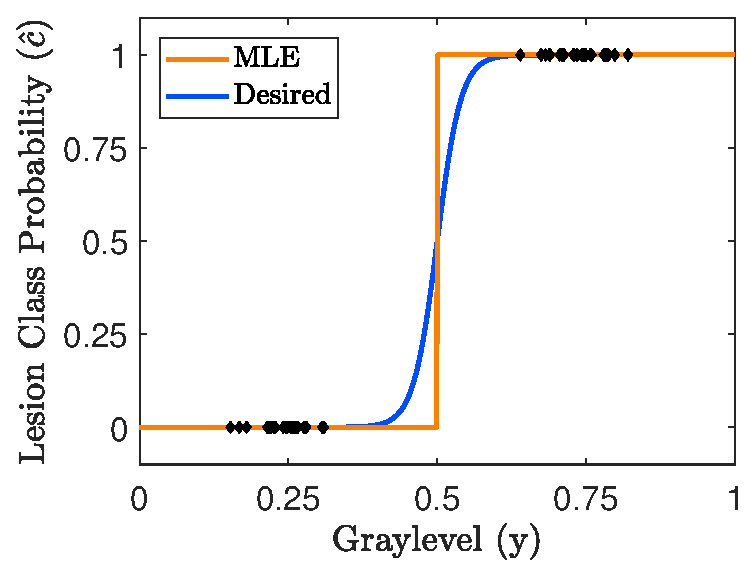
\includegraphics[width=\textwidth]{chmle-sep}\caption{Separable classes}\label{fig:chmle-sep}
  \end{subfigure}
  \begin{subfigure}{\plotwidth}
    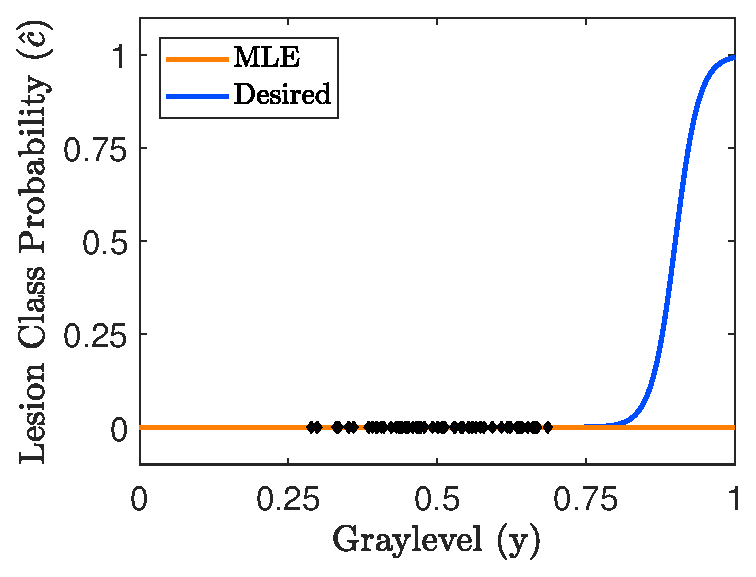
\includegraphics[width=\textwidth]{chmle-noles}\caption{No lesions}\label{fig:chmle-noles}
  \end{subfigure}
  \caption{Challenges encountered during estimation of a logistic model.}
  \label{fig:chmle}
\end{figure}
% --------------------------------------------------------------------------------------------------
\subsubsection{Joint Estimation}
In the LPA algorithm, the logistic feature weights for each voxel are not considered independent. The FLAIR graylevel effect is tied across all voxels -- i.e. $\b^1(x) \rightarrow \b^1$, so $\eta(x) = \b^0(x) + \b^1Y(x)$ -- and a Gaussian MRF model is used to estimate the spatially varying intercept $\b^0(x)$. This design addresses the aforementioned challenges by greatly increasing the number of observations used to estimate each parameter. However, it requires joint estimation of all parameters simultaneously, and dramatically increases the complexity of estimation \cite{Schmidt2017a}.
\par
Efficient fitting of such models was the subject of major works by \citeauthor{Schmidt2017} \cite{Schmidt2017,Schmidt2017a}, but several drawbacks remain.
First, Markov Chain Monte Carlo estimation of the model appears to create discontinuity artifacts in the spatial effect image $\b^0(x)$, as shown in Figure \ref{fig:B-lpa}.
Second, MRF modelling of the parameter images assumes that the missing data (i.e. WMH training examples in the more superficial brain regions) can be interpolated spatially, but this may not be justified.
Third, the proposed joint estimation procedures are computationally expensive (versus the methods proposed here), requiring approximately two hours to estimate $\bb(x)$ \cite{Schmidt2017a}.
Finally, it is not clear whether any tied $\b$ are necessary or advantageous in this context.
These deficiencies then motivate investigations into alternative solutions to the above challenges.
\par
In addition to these potential modelling weaknesses, there were also several limitations to the validation methodology for the LPA algorithm, worth noting here.
First, the ``ground truth'' segmentations were generated using an automated algorithm -- the Lesion Growth Algorithm (LGA) \cite{Schmidt2012} of the same toolbox -- rather than a human expert.
Second, the graylevel standardization procedure employed does not consider the variance of image graylevels (only the mean is subtracted); this strongly assumes that user images will have graylevels spanning a similar range.
Third, all 53 training cases were obtained on the same MRI scanner, which may limit generalization performance.
Finally, no segmentation performance results are given in either of the associated publications \cite{Schmidt2017,Schmidt2017a}.
Therefore, while the open-source release of the LPA algorithm is greatly appreciated, significant improvements can be made to this algorithm.
% --------------------------------------------------------------------------------------------------
\subsubsection{Independent Estimation}
An alternative approach is to consider each parameter vector $\bb(x)$ independent. Doing so greatly simplifies model fitting, but does not address the challenges described above. These must instead be addressed using regularization strategies, as discussed below in \S\ \ref{s:reg-method}. In this section, ML estimation of independent parameter vectors $\bb$ is developed. For clarity, only a single voxel is considered -- i.e. $y$ from $Y(x)$, etc.
\par
As note above, the optimal $\bb$ for each independent voxel can be resolved using MLE. If the training data are also assumed to be independently observed, then the likelihood (conditioned on the data) is defined from binomial theory as
\begin{align}
  L(\bb\mid\C,\bY) &= \prod_{n=1}^{N} P(c=1\mid\by_n,\bb)^{c_n} \left(1-P(c=1\mid\by_n,\bb)^{1-c_n}\right)\nonumber\\
  &= \prod_{n=1}^{N} \Big[\hat{c}_n^{\en c_n} \left(1-\hat{c}_n^{\en 1-c_n}\right)\Big].
  \label{eq:likelihood}
\end{align}
For computational reasons, it is simpler and asymptotically equivalent to maximize the log-likelihood,
\begin{align}
\L(\bb) &= \log{ \prod_{n=1}^{N} \Big[\hat{c}_n^{\en c_n} \left(1-\hat{c}_n^{\en 1-c_n}\right)\Big] }\nonumber\\
&= \sum_{n=1}^{N} \Big[ c_n \log \hat{c}_n + (1-c_n) \log (1-\hat{c}_n) \Big] \nonumber\\
&= \sum_{n=1}^{N} \Big[ c_n \bb^T\by_n - \log (1+e^{\bb^T\by_n}) \Big].
\label{eq:loglikelihood}
\end{align}
The optimal $\bb$ is therefore resolved by maximizing the log-likelihood,
\begin{align}
\bb^* &= \underset{\bb}{\arg\max} \en\L(\bb)\nonumber\\
&= \underset{\bb}{\arg\max}\en\sum_{n=1}^{N} \Big[ c_n \bb^T\by_n - \log (1+e^{\et\bb^T\by_n}) \Big]
\label{eq:argmaxmle}
\end{align}
% --------------------------------------------------------------------------------------------------
\subsubsection{Iterative Updates}
Estimation of $\bb^*$ can be performed using iterative optimization, using an initial estimate $\bb^{(0)}$ and an update term $\Delta\bb^{(t)}$,
\begin{equation}
\bb^{(t+1)} \leftarrow \bb^{(t)} + \alpha\thinspace\Delta\bb^{(t)},
\label{eq:update}
\end{equation}
where $\alpha$ is a small valued learning rate parameter. There are many possible definitions of $\Delta\bb$, including simply the gradient of $\L(\bb)$, denoted $\nabla_{\bb}\L$. However, it can be shown that $\L(\bb)$ is convex, so higher order update equations can be used. The work by \citeauthor{Minka2003} \cite{Minka2003} compares several options, including Newton's method (and variants), conjugate gradient, iterative scaling (and variants), and dual optimization%
\footnote{Matlab code available at \hreftt{https://github.com/tminka/logreg/}}.
For small feature dimensionality ($K$), performance differences among the options were small. Classic Newton updates gave a good balance between memory requirements and computational order, so they are used.
\par
If the gradient $\nabla_{\bb}\L$ and Hessian matrix $\nabla^2_{\bb}\L$ are defined as
\begin{align}
\nabla_{\bb}\L &= \left[\begin{array}{c}
\frac{\d L}{\d\b^1}\\\vdots\\\frac{\d L}{\d\b^\K}
\end{array}\right],\label{eq:llgradient0}\\
\nabla^2_{\bb}\L &= \left[\begin{array}{ccc}
\frac{\d^2 L}{\d\b^1\d\b^1}&\cdots&\frac{\d^2 L}{\d\b^1\d\b^\K}\\
\vdots&\ddots&\vdots\\
\frac{\d^2 L}{\d\b^\K\d\b^1}&\cdots&\frac{\d^2 L}{\d\b^\K\d\b^\K}
\end{array}\right]\label{eq:llhessian0},
\end{align}
then the Newton update is given by
\begin{equation}
\Delta\bb = -{\nabla^2_{\bb}\L}^{-1}\nabla_{\bb}\L.
\label{eq:newtonmle}
\end{equation}
In the current model, the gradient is given by 
\begin{equation}
\nabla_{\bb}\L = \sum_{n=1}^{N} \by_n\left(c_n - \hat{c}_n\right),
\label{eq:llgradient}
\end{equation}
and the Hessian by
\begin{equation}
\nabla^2_{\bb}\L = \sum_{n=1}^{N} \by_n{\by_n}^T \left(c_n - \hat{c}_n\right).
\label{eq:llhessian}
\end{equation}
Substituting (\ref{eq:llgradient}) and (\ref{eq:llhessian}) into (\ref{eq:newtonmle}), the explicit update  $\Delta\bb$ for (\ref{eq:update}) is obtained.
% --------------------------------------------------------------------------------------------------
\subsubsection{Implementation}
Speed of model fitting is a significant factor during development, particularly considering optimization of so-called hyperparameters. Faster training yields more model iterations, which inevitably bear improvements. While the above estimation procedure must be repeated for the voxels of interest in the standardized space, there are several ways of accelerating this procedure.
\par
First, it is prudent to only estimate the parameters for voxels in the brain. These voxels can be selected using a ``brain mask'', denoted $M(x)$ -- a binary image denoting the expected location of the brain in standardized space (c.f. \S\ \ref{ss:brainmask} for details about the brain mask used in this work).
\par
% __JK__ does this (below) belong in the appendix?
Second, since every estimation is independent in the current model, it is possible to compute these in parallel. To do so, the training data must be vectorized with respect to spatial location $x$, and the matrix operations outlined above must be expanded explicitly to accommodate the new dimension. To begin, the training data from all subjects -- features $\bm{\Y}(x)$, with $\Y^0=1$, and labels $\C(x)$ -- are sampled from nonzero locations in the MNI-space brain mask. These data are stored in two matrices $\x{Y}$ and $\x{C}$, with dimensions $[V,N,K+1]$ and $[V,N,1]$, respectively, where $V$ is the total number of nonzero voxels in the brain mask, $N$ is the number of subjects, and $K$ is the number of features. A similar matrix is constructed for the initial parameters $\bb^{(0)}(x)$, denoted $\x{B}^{(0)}$, with dimensions $[V,1,K+1]$. Let $\x{Y}_n^k$ denote the vector of data from all voxels for the $k$\ss{th} feature from the $n$\ss{th} subject, and so on for $\x{C}$ and $\x{B}$.
\par
% damn it: have not yet introduced lambda yet here... how to resolve this?
% need a smoother transition here.
In order to simplify subsequent calculations, the feature data are rectified according to the class labels, before the first iteration, as in
\begin{equation}
\x{Y}_n^k =
\begin{cases}
+\x{Y}_n^k, & \x{C}_n \ge 0.5\\
-\x{Y}_n^k, & \x{C}_n <  0.5\\
\end{cases},\qquad\forall\et k \in \{1,\dots,K\}.
\end{equation}
Next, for a given iteration $t$, the following vectorized calculations yield the update matrix $\Delta\x{B}^{(t)}$.
Regarding notation:
1) the iteration index ${}^{(t)}$ is omitted for clarity,
2) element-wise multiplication is denoted by $\circ$, and
3) the variable $K$ is now defined as $1$, since this is essential to the simplification.
\begin{align}
\x{S} &= \frac{1}{1+e^{\et\eta}},\qquad \eta = \x{B}^0 + \left(\x{B}^1\ep\x{Y}^1\right)\\
\x{A} &= \x{S}\ep\left(1-\x{S}\right)\\
\x{G} &= \nabla_{\x{B}}\L - \lambda\x{B} \nonumber \\
&= \left[\begin{array}{c}
\x{G}^1 \\ \x{G}^2
\end{array}\right] \nonumber \\
&= \left[\begin{array}{c}
\sum_{n=1}^{N}\left( \x{Y}_n^1\circ\x{S} \right) \\
\sum_{n=1}^{N}\left( \x{Y}_n^2\circ\x{S} \right)
\end{array}\right] - \lambda\left[\begin{array}{c} \x{B}^1 \\ \x{B}^2\end{array}\right]\\
\x{H} &= \nabla_{\x{B}}^2\L -\lambda\x{I} \nonumber \\
&= \left[\begin{array}{cc}
\x{H}^{1,1} & \x{H}^{1,2} \\ \x{H}^{2,1} & \x{H}^{2,2}
\end{array}\right] \nonumber \\
&= \left[\begin{array}{cc}
\sum_{n=1}^{N}\left( \x{A}\circ\x{Y}_n^1\circ\x{Y}_n^1 \right) & 
\sum_{n=1}^{N}\left( \x{A}\circ\x{Y}_n^2\circ\x{Y}_n^1 \right) \\
\sum_{n=1}^{N}\left( \x{A}\circ\x{Y}_n^1\circ\x{Y}_n^2 \right) & 
\sum_{n=1}^{N}\left( \x{A}\circ\x{Y}_n^2\circ\x{Y}_n^2 \right)
\end{array}\right] - \lambda\left[\begin{array}{cc} 1 & \\ & 1\end{array}\right]\\
\x{D} &= \det{\x{H}} \nonumber \\
&= \left(\x{H}^{1,1}\circ\x{H}^{2,2}\right) - \left(\x{H}^{1,2}\circ\x{H}^{2,1}\right) \\
\Delta\x{B} &= -\x{H}^{-1}\x{G} \nonumber \\
&= \dfrac{1}{\x{D}} \left[\begin{array}{cc}
\left(\x{H}^{2,2}\circ\x{G}^{1} - \x{H}^{2,1}\circ\x{G}^{2} \right) & 
\left(\x{H}^{1,2}\circ\x{G}^{2} - \x{H}^{1,1}\circ\x{G}^{1} \right)
\end{array}\right]^{T}
\end{align}
\par...\par
Finally, 
%%%%%%%%%%%%%%%%%%%%%%%%%%%%%%%%%%%%%%%%%%%%%%%%%%%%%%%%%%%%%%%%%%%%%%%%%%%%%%%%%%%%%%%%%%%%%%%%%%%%
\section{Regularization}\label{s:reg-method}
Regularizations are methods of injecting prior knowledge about the expected model into the optimization. Assuming voxel-wise independence of model parameters requires the use of regularization strategies to solve the challenges outlined in \S\ \ref{ss:modelfitting}. Model fitting which includes regularization is termed maximum a posteriori (MAP) estimation. Several regularization methods are explored below.
% ==================================================================================================
\subsection{Data Augmentation}
Noting the central role of training data in each of the challenges, methods of artificially increasing the training dataset size may be particularly useful in solving them. Data augmentation has long been used in machine learning tasks with limited training data, and there are several methods of generating synthetic data. In low dimensional input/output spaces, random sampling of fitted class-conditional posterior distributions can produce reasonable samples with known labels \cite{Tanner1987}. In higher dimensional problem spaces, however, imputation is more difficult \cite{Goodfellow2014}. For example, the space of potential $100\times100\times100$-sized images has $100^3$ dimensions (one per voxel), yet only a small inner subspace represents plausible images. Generating synthetic examples in this space is therefore challenging, especially for segmentation tasks, where the outputs have dimensionality roughly equal to the input.
\par
Alternatively, simple image manipulations can still afford model improvements \cite{Krizhevsky2012}. In segmentation tasks, both the input image(s) and the corresponding label images can be translated, reflected, rotated, and perhaps resized, thereby avoiding the generation of genuinely synthetic examples. In the current work, reflections and small (one-voxel) translations can be applied to the label and FLAIR images following registration to the MNI brainspace.
% ==================================================================================================
\subsection{Classic Regularization}
The separable classes challenge is well-known in regression problems, and a good solution is to penalize the magnitude of model parameters using the $L_p$-norm: $\lambda\norm{\bb}_p$ \cite{Zou2005}. It can be shown that $L_1$ regularization corresponds to a Laplacian prior on elements of $\bb$, with scale parameter inversely proportional to $\lambda$ (equivalently, this assumes that the model error follows this distribution); similarly, $L_2$ regularization implies a Gaussian prior, with standard deviation inversely proportional to $\lambda$ \cite{Zou2005}. This penalty can then be appended to the objective function (\ref{eq:argmaxmle}), as in 
\begin{align}
\bb^* &= \J(\bb)\nonumber\\
&= \underset{\bb}{\arg\max}\en\L(\bb) - \lambda\norm{\bb}_p \nonumber\\
&= \underset{\bb}{\arg\max}\en\sum_{n=1}^{N} \Big[ c_n \bb^T\by_n - \log (1+e^{\et\bb^T\by_n}) \Big] - \lambda\norm{\bb}_p
\label{eq:argmaxmap}
\end{align}
Due to its relatively large gradient near zero, $L_1$ regularization is typically used to encourage sparsity in the feature weights (i.e. $\b^k\rightarrow0$) \cite{Tibshirani1996}. This is not desirable in the current model, since the feature (FLAIR graylevel) is known to be discriminative. Moreover, the expansion of the $\norm{\bb}_1$ term in the gradient of the objective function is not straightforward, since it is non-differentiable at zero \cite{Tibshirani1996,Lee2006}. Conversely, $L_2$ regularization is more effective at limiting parameter magnitude -- which is the current aim -- and the first and second order gradients of (\ref{eq:argmaxmap}) derive easily \cite{Minka2003}. For these reasons, only $L_2$ regularization is considered, yielding the following change to the Newton update expression (\ref{eq:newtonmle}),
\begin{equation}
\Delta\bb = -{\left(\nabla^2_{\bb}\L-\lambda I\right)}^{-1}\left(\nabla_{\bb}\L-\lambda\bb\right)
\label{eq:newtonmap}
\end{equation}
What remains is to select an appropriate value of $\lambda$. This is explored experimentally in \S\ \ref{ss:toyreg} using a toy model.
% ==================================================================================================
\subsection{Pseudo-Lesions}
The Sparsely observed lesion class challenge is less common, since discriminative models are rarely fit in the absence of one class altogether. This occurs here because all voxels are modelled independently. It is therefore tempting to simply sample features (FLAIR graylevels) from the lesion class at other spatial locations in order to fit the logistic model in the healthy training voxels. However, as noted in \S\ \ref{ss:autochallenges} and \S\ \ref{s:modelconcept}, there may be spatially-correlated heterogeneity in the appearance of lesions \cite{Sled2004,Stevenson2000}, and some locations will likely never contain any lesion. Considering these facts, generating additional synthetic lesion-class samples, or ``pseudo-lesions'', for these locations using static, spatially parameterized definitions would have two advantages. First, this approach would not be subject to variations in the training data. Second, it would be feasible to consider the prior probability of healthy tissues (GM / WM / CSF) in the definition.
\par...\par
% ==================================================================================================
\subsection{Parameter Image Smoothing}
Finally, 
\par...\par
While an alternative approach might involve modelling the parameter images as a spatial function (e.g. band-limited discrete cosine / Fourier transform), there are two challenges with this approach.
First, deriving the update gradients for such a model would be challenging, and their computation might increase training time.
Second, such an encoding may introduce artifacts in the resulting parameter images.
Moreover, it is well known that frequency domain band-limiting can be equivalently achieved by convolution (i.e. filtering) in the spatial domain \cite{Gonzalez2006}.
\par...\par
\citeauthor{Harmouche2015} \cite{Harmouche2015} also note that in smoothly varying models, small registration errors can be expected to have only a minor impact.
%%%%%%%%%%%%%%%%%%%%%%%%%%%%%%%%%%%%%%%%%%%%%%%%%%%%%%%%%%%%%%%%%%%%%%%%%%%%%%%%%%%%%%%%%%%%%%%%%%%%
\section{Bias Correction \& Registration}
Two objectives of preprocessing 
\par...\par
%%%%%%%%%%%%%%%%%%%%%%%%%%%%%%%%%%%%%%%%%%%%%%%%%%%%%%%%%%%%%%%%%%%%%%%%%%%%%%%%%%%%%%%%%%%%%%%%%%%%
\section{Graylevel Standardization}
\par...\par
\clearpage
%%%%%%%%%%%%%%%%%%%%%%%%%%%%%%%%%%%%%%%%%%%%%%%%%%%%%%%%%%%%%%%%%%%%%%%%%%%%%%%%%%%%%%%%%%%%%%%%%%%%
\section{Post-Processing}

\clearpage
%%%%%%%%%%%%%%%%%%%%%%%%%%%%%%%%%%%%%%%%%%%%%%%%%%%%%%%%%%%%%%%%%%%%%%%%%%%%%%%%%%%%%%%%%%%%%%%%%%%%
\section{Performance Metrics}
\label{ss:metrics}
Segmentation performance of the model is characterized in two respects: voxel-wise agreement and total lesion load (LL) volume agreement. 
When comparing the estimated segmentation ($\hat{c}$) to the ground truth segmentation ($c$), each individual voxel can occupy one of four states (colours shown for future reference):
\begin{itemize}[itemsep=0pt]
  \item[\textcolor{green}{\scalebox{0.7}{$\blacksquare$}}] True Positive (TP): $c = 1$ and $\hat{c} = 1$, correctly predicted ``lesion''.
  \item[\textcolor{red}  {\scalebox{0.7}{$\blacksquare$}}] False Positive (FP): $c = 0$ and $\hat{c} = 1$, incorrectly predicted ``lesion''.
  \item[\textcolor{blue} {\scalebox{0.7}{$\blacksquare$}}] False Negative (FN): $c = 1$ and $\hat{c} = 0$, incorrectly predicted ``healthy''.
  \item[\textcolor{black}{\scalebox{0.7}{$\blacksquare$}}] True Negative (TN): $c = 0$ and $\hat{c} = 0$, correctly predicted ``healthy''.
\end{itemize}
Summing the number of voxels in each state, voxel-wise agreement can then be quantified using the following measures:
\begin{itemize}
  \item \textbf{Similarity Index (SI)} (\textsc{aka} Dice Similarity Coefficient, F1-Score)\\Measures overall segmentation performance.
  \begin{equation}SI = \dfrac{2TP}{2TP + FP + FN}\end{equation}
  \item \textbf{Precision (Pr)} (\textsc{aka} Overlap Fraction, Positive Predictive Value)\\Fraction of predicted predicted positives which are true positives.
  \begin{equation}Pr = \dfrac{TP}{TP+FP}\end{equation}
  \item \textbf{Recall (Re)} (\textsc{aka} Sensitivity, True Positive Rate)\\Fraction of true positives which are predicted positive.
  \begin{equation}Re = \dfrac{TP}{TP+FN}\end{equation}
\end{itemize}
Each measure is $\in [0,1]$, where higher is better. Note that typical performance metrics like accuracy and sensitivity are avoided, since they include the $TN$ count in the numerator, which is typically much larger than $TP + FP + FN$ combined (i.e. $c=1$ is a rare event).
\par
Overall volume agreement between segmentations is characterized using the 2-way mixed-effects single-rater absolute intraclass correlation coefficient (ICC)%
\footnote{Option \texttt{`A-1'} in the Matlab function \texttt{ICC} from \hreftt{https://www.mathworks.com/matlabcentral/fileexchange/22099}}\ 
\cite{Koo2016}, while trends in over/undersegmentation with lesion load are illustrated using Blant-Altman plots \cite{Altman1983}.
%%%%%%%%%%%%%%%%%%%%%%%%%%%%%%%%%%%%%%%%%%%%%%%%%%%%%%%%%%%%%%%%%%%%%%%%%%%%%%%%%%%%%%%%%%%%%%%%%%%%
\section{Model Summary}



A summary of the model is shown in Figure \ref{fig:modelsum}.
\begin{figure}
  \centering\scalebox{0.65}{\pgfdeclarelayer{background}
\pgfdeclarelayer{foreground}
\pgfsetlayers{background,main,foreground}
\tikzset{%
  arrow/.style = { ->, >=Latex,  very thick, rounded corners, draw = #1!60!white },
  input/.style = { ->, >=Latex, ultra thick, rounded corners, draw = red },
  clr/.style   = { ultra thick, rounded corners, fill = #1!60!white },
  image/.style = { fill = black, draw = black!80!white, ultra thick, inner sep = 0 },
  plot/.style  = { fill = white, inner sep = 0 },
  label/.style = { fill = white, fill opacity = 0, text opacity = 1 },
  tbox/.style  = { fill = white, draw = #1!60!white, very thick, align = center }
}
\newcommand*{\img}[3]{%
  \node[image] at (#1,#2){\includegraphics[width=\ixx cm, height=\iyy cm]{#3}}; % chktex 1
}
\newcommand*{\imgt}[4]{%
	\img{#1}{#2}{#3}
	\begin{pgfonlayer}{foreground}
		\node[label] at (#1,#2-\iy-0.4){\large #4};
	\end{pgfonlayer}
}
\newcommand*{\plot}[5]{%
  \node[plot] at (#1,#2){\includegraphics[width=#3cm, height=#4cm]{#5}};
}
\newcommand*{\voxpath}[4]{%
  \filldraw[fill=black!20!white,draw=black]
  (#1,#2)--(#1+\vw,#2)--(#1+#3,#2-#3+\vw)--(#1+#3-\vw,#2-#3+\vw)--(#1,#2);
  \filldraw[fill=black!20!white,draw=black]
  (#1,#2)--(#1,#2-\vw)--(#1+#3-\vw,#2-#3)--(#1+#3-\vw,#2-#3+\vw)--(#1,#2);
  \filldraw[fill=black!20!white,draw=black]
  (#1+#3,#2-#3)--(#1+#3,#2-#3+\vw)--(#1+#3-\vw,#2-#3+\vw)--(#1+#3-\vw,#2-#3)--(#1+#3,#2-#3);
  \node[below right] at (#1+#3,#2-#3) {#4};
}
\newcommand*{\imgstack}[5]{%
  \foreach \x in {0,...,#3}{\img{#1-0.1*#3+0.1*\x}{#2+0.1*#3-0.1*\x}{#4}} % chktex 11 chktex 1
  \begin{pgfonlayer}{foreground}
	  \node[label] at (#1,#2-\iy-0.4){\large #5};
	\end{pgfonlayer}{foreground}
}
\newcommand*{\imgvoxstack}[5]{%
	\voxpath{#1+\vw+0.3-0.1*#3-\vl-\vl}
					{#2-\vw-0.2+0.1*#3+\vl+\vl}{\vl}{}
	\imgstack{#1}{#2}{#3}{#4}{#5}
	\voxpath{#1+\vw+0.3}
	        {#2-\vw-0.2}{\vl}{}
}
\newcommand*{\textbox}[6]{%
  \node[tbox=#5,minimum width=#3cm,minimum height=#4cm]at(#1,#2){#6};
}
%\newcommand*{\blocktitle}[4]{%
%  \node[title=#3]at(#1,#2){#4};
%  \fill[clr=#3](#1+0.6,#2+1.7)--(#1+0.6,#2-1.7)--(#1+0.6+0.3,#2);
%}
\newcommand*{\vw}{0.1}
\newcommand*{\vl}{0.7}
\newcommand*{\ix}{0.8}\newcommand*{\ixx}{1.6}
\newcommand*{\iy}{1}  \newcommand*{\iyy}{2}
\newcommand*{\pw}{1.5}
\newcommand*{\fw}{0.3}

% --------------------------------------------------------------------------------------------------
\begin{tikzpicture}
    \useasboundingbox(1.5, 0.0) rectangle (24.0, 20.5);
    \begin{pgfonlayer}{background}
      % background boxes
      \draw[black!30!white,rounded corners,very thick](-0.25, 0.25) rectangle (23.75, 9.75);
      \draw[black!30!white,rounded corners,very thick](-0.25,10.25) rectangle (23.75,20.00);
      % box labells
      \node[fill=black!10!white,rounded corners,minimum width=3cm, minimum height=1.0cm]
        at(21.75,19.00){\textsc{Training}};
      \node[fill=black!10!white,rounded corners,minimum width=3cm, minimum height=1.0cm]
        at(21.75, 8.75){\textsc{Testing}};
      %\draw[step=0.5,black!10!white,very thin](-0.5, 0.0) grid (24.0,20.0);
    \end{pgfonlayer}
    % training
    \imgt       { 1.0}{18.0}{c1}{$\mathrm{C}_1(x)$}
    \imgt       { 1.0}{14.0}{c2}{$\mathrm{C}_{\textsc{n}}(x)$}
    \imgt       { 3.0}{18.0}{i1}{$\mathrm{Y}_1(x)$}
    \imgt       { 3.0}{14.0}{i2}{$\mathrm{Y}_{\textsc{n}}(x)$}
    \node[font=\fontsize{30}{0}\selectfont,align=center] at ( 1.0,15.8) {$\vdots$};
    \node[font=\fontsize{30}{0}\selectfont,align=center] at ( 3.0,15.8) {$\vdots$};
    \imgstack   {10.0}{16.0}{6}{ir} {$\mathcal{Y}(x)$}
    \imgvoxstack{13.0}{16.0}{6}{jr} {$\tilde{\mathcal{Y}}(x)$}
    \imgvoxstack{13.0}{12.0}{6}{c1} {$\mathcal{C}(x)$}
    \plot       {17.5}{14.0}{4}{4}  {lr-fit}
    \imgvoxstack{22.0}{14.0}{1}{bb} {$\bm{\beta}(x)$}
    % testing
    \imgstack   { 3.0}{ 2.0}{1}{bb} {$\bm{\beta}(x)$}
    \imgvoxstack{ 3.0}{ 6.0}{0}{it} {$Y_{test}(x)$}
    \imgvoxstack{10.0}{ 2.0}{1}{bb} {$\bm{\upbeta}(x)$}
    \imgvoxstack{10.0}{ 6.0}{0}{jt} {$\tilde{\mathrm{Y}}_{test}(x)$}
    \plot       {14.5}{ 4.0}{4}{4}  {lr-test}
    \imgvoxstack{19.0}{ 4.0}{0}{qt} {$\hat{\mathrm{C}}_{test}(x)$}
    \imgt       {22.0}{ 4.0}{lt}    {$\hat{\mathrm{C}}_{test}^{\circ}(x)$}
    % training arrows
    \draw[arrow={blue}  ]( 3.0+\ix,18.0    )--( 3.5+\ix,18.0)--( 3.5+\ix,16.0)--( 5.0,16.0);
    \draw[arrow={blue}  ]( 3.0+\ix,16.0    )--( 5.0    ,16.0);
    \draw[arrow={blue}  ]( 3.0+\ix,14.0    )--( 3.5+\ix,14.0)--( 3.5+\ix,16.0)--( 5.0,16.0);
    \draw[arrow={blue}  ]( 8.0    ,16.0    )--(10.0-\ix,16.0);
    \draw[arrow={blue}  ]( 1.0    ,12.3    )--( 1.0    ,12.0)--( 5.0,    12.0);
    \draw[arrow={blue}  ]( 5.0    ,12.0    )--(13.0-\ix,12.0);
    \draw[arrow={blue},dotted](6.5,16.0    )--( 6.5    ,12.5);
    \draw[arrow={violet}](10.0    ,16.0+\iy)--(10.0    ,18.5);
    \draw[arrow={violet}](11.5,    19.0    )--(13.0    ,19.0)--(13.0,16.0+\iy);
    \draw[arrow={red}   ](13.0+\ix,16.0    )--(14.5    ,16.0)--(14.5,14.0)--(15.5,14.0);
    \draw[arrow={red}   ](13.0+\ix,12.0    )--(14.5    ,12.0)--(14.5,14.0)--(15.5,14.0);
    \draw[arrow={red}   ](19.5    ,14.0    )--(22.0-\ix,14.0);
    % testing arrows
    \draw[arrow={blue}  ]( 3.0+\ix, 6.0    )--( 5.0    , 6.0);
    \draw[arrow={blue},dotted](6.5, 6.0    )--( 6.5    , 2.5);
    \draw[arrow={blue}  ]( 3.0+\ix, 2.0    )--( 5.0    , 2.0);
    \draw[arrow={blue}  ]( 8.0    , 2.0    )--(10.0-\ix, 2.0);
    \draw[arrow={violet}]( 6.5    , 6.5    )--( 6.5    , 8.0);
    \draw[arrow={violet}]( 8.0    , 8.5    )--(10.0    , 8.5)--(10.0    , 6.0+\iy);
    \draw[arrow={red}   ](10.0+\ix, 6.0    )--(11.5    , 6.0)--(11.5, 4.0)--(12.5, 4.0);
    \draw[arrow={red}   ](10.0+\ix, 2.0    )--(11.5    , 2.0)--(11.5, 4.0)--(12.5, 4.0);
    \draw[arrow={red}   ](16.5    , 4.0    )--(19.0-\ix, 4.0);
    \draw[arrow={orange}](19.0    , 4.0+\iy)--(19.0    , 6.5);
    \draw[arrow={orange}](20.5,     7.0    )--(22.0    , 7.0)--(22.0, 4.0+\iy);
    % training texts
    \textbox    { 6.5}{16.0}{3}{1.0}{blue}  {Bias Correction\\\& Registration}
    \textbox    { 6.5}{12.0}{3}{1.0}{blue}  {Same Transform\\Applied}
    \textbox    {10.0}{19.0}{3}{1.0}{violet}{Histogram\\Matching}
    \textbox    {17.5}{17.0}{4}{1.0}{red}   {Logistic Regression\\Model Fitting}
    % testing texts
    \textbox    { 6.5}{6.25}{3}{0.5}{blue}  {Bias Correction}
    \textbox    { 6.5}{5.75}{3}{0.5}{blue}  {Registration}
    \textbox    { 6.5}{ 2.0}{3}{1.0}{blue}  {Inverse Transform\\Applied}
    \textbox    { 6.5}{ 8.5}{3}{1.0}{violet}{Histogram\\Matching}
    \textbox    {14.5}{ 7.0}{4}{1.0}{red}   {Logistic Regression\\Lesion Prediction}
    \textbox    {19.0}{ 7.0}{3}{1.0}{orange}{Post\\Processing}
\end{tikzpicture}}
  \caption{Overview of the proposed algorithm. Typefaces -- upright Roman: images in native space; italic Roman: images in standard (MNI) space; calligraphic: a set of images from several patients; bold: a set of images corresponding to different features; Variables -- $C(x)$: manual segmentation; $Y(x)$: FLAIR image, $\beta(x)$: parameter image; $\hat{C}(x)$: estimated lesion segmentation.}
  \label{fig:modelsum}
\end{figure}
% ==================================================================================================
\subsection{Tunable Parameters}
In order to achieve the best possible model performance, it is prudent to track tunable model parameters (\textsc{aka} hyperparameters) which are distinct from those fitted during each cross validation fold. Considering both the main VLR model and the pre- and post-processing aspects, the parameters of the proposed algorithm are summarized in Table \ref{tab:hyperparams}. The optimization of these model components will be the subject of the next chapter. 
%and also programmatically in \nameref{code:hypdef}.
\begin{table}
  \centering
  \caption{Model hyperparameters.}
  \label{tab:hyperparams}
  \begin{tabular}{lllll}
    \hline
    Stage                            & Parameter            & Notation                    & Type                                          & Default                   \\ \hline
    \multirow{4}{*}{Pre-Processing}  & Reflect Augmentation & $A_R$                       & $\mathbb{B}$                                  & 0                         \\
                                     & Shift Augmentation   & $A_S$                       & $\mathcal{N}_p$                                        & $\mathcal{N}_0$                    \\
                                     & Graylevel Transform  & $T_y$                       & $f: y\mapsto \tilde{y}$                       & $f_{he}$                  \\
                                     & Transform Mask       & $M_{T}(x)$                  & $\mathbb{B}(x)$                               & $M_{\text{brain}}$        \\ \hline
    \multirow{6}{*}{VLR Fitting}     & Iterations           & $N_{t}^{\lr}$               & $\mathbb{Z}$                                  & 30                        \\
                                     & Initial $\bb$        & $\bb^{(0)}$                 & $\Re^2$                                       & $[0,0]$                   \\
                                     & Learning Rate        & $\alpha$                    & $\Re$                                         & 1                         \\
                                     & Regularization       & $\lambda$                   & $\Re$                                         & 0                         \\
                                     & Pseudo-Lesions       & $\{\bY_{\rho},\bC_{\rho}\}$ & $\{\{\et\cdot\in\Re\},\{\et\cdot\in[0,1]\}\}$ & $\{\{\},\{\}\}$           \\
                                     & $\bb$ Filter         & $F_{\bb}$                   & $f: \bb(\mathcal{N}_p(x)) \mapsto \tilde{\bb}(x)$      & $\tilde{\bb}(x) = \bb(x)$ \\ \hline
    \multirow{3}{*}{Post-Processing} & Min Lesion  Size     & $\X_{\min}^{c}$             & $\Re\en(\text{mm}^{3})$                       & 0                         \\
                                     & MRF Iterations       & $N_{t}^{\mrf}$              & $\mathbb{Z}$                                  & 0                         \\
                                     & MRF Weights          & $W_{\mrf}$                  & $\{w_{\Delta},w_{F},w_y\}$                    & $\{1,1,1\}$               \\ \hline
  \end{tabular}
  \tablepost{Notation. $\mathbb{B}$: boolean value; $\mathbb{Z}$: integer value; $\mathbb{R}^n$: real value ($n=1$) or vector ($n > 1$); $\mathcal{N}_p$: nearest $p$ voxel neighbourhood.}
\end{table}
% --------------------------------------------------------------------------------------------------
% ==================================================================================================
%%%%%%%%%%%%%%%%%%%%%%%%%%%%%%%%%%%%%%%%%%%%%%%%%%%%%%%%%%%%%%%%%%%%%%%%%%%%%%%%%%%%%%%%%%%%%%%%%%%%
